\documentclass[12pt, titlepage]{article}

\usepackage{fullpage}
\usepackage[round]{natbib}
\usepackage{multirow}
\usepackage{booktabs}
\usepackage{tabularx}
\usepackage{graphicx}
\usepackage{float}
\usepackage{hyperref}
\hypersetup{
    colorlinks,
    citecolor=black,
    filecolor=black,
    linkcolor=red,
    urlcolor=blue
}
\usepackage[round]{natbib}

\newcounter{acnum}
\newcommand{\actheacnum}{AC\theacnum}
\newcommand{\acref}[1]{AC\ref{#1}}

\newcounter{ucnum}
\newcommand{\uctheucnum}{UC\theucnum}
\newcommand{\uref}[1]{UC\ref{#1}}

\newcounter{mnum}
\newcommand{\mthemnum}{M\themnum}
\newcommand{\mref}[1]{M\ref{#1}}

\title{SE 3XA3: \color{red}Module Guide\color{black}\\Shuffle}

\author{Team 16, AsK Studios
		\\ Aidan Schonewille, schonea
		\\ Sullivan Stobo, stobos1
		\\ Karlo Delalic, delalik
}

\date{\today}


\begin{document}

\section*{Revision History}
\begin{center}
\begin{tabular}{| c | c | p{6cm} |}
\hline
\textbf{Date} & \textbf{Developer(s)} & \textbf{Change}\\
\hline
October 6, 2017 & Aidan/Sullivan/Karlo & Initial creation of document.\\
\hline
December 5, 2017 & Sullivan & Finalized \\
\hline
\end{tabular}
\end{center}

\maketitle

\pagenumbering{roman}
\tableofcontents
\listoftables
\listoffigures

\newpage

\pagenumbering{arabic}

\section{Introduction}

\color{red} The purpose of this document is to outline the various modules that the project 'Shuffle' is divided into.  The practice of dividing software is to various modules is very common as it allows the program to be viewed in smaller parts, which can make it easier to understand.  It also makes it easier to trace issues and add features. \color{black}

\section{Anticipated and Unlikely Changes} \label{SecChange}

\color{red}This section lists any changes that may be made to the system.  They are categorized according to likeliness.  Anticipated changes list likely changes, while Unlikely changes list unlikely changes\color{black}

\subsection{Anticipated Changes} \label{SecAchange}

\color{red}These changes would likely require only changing one module, making them simple to implement without massively altering the system. \color{black}

\begin{description}
\item[\refstepcounter{acnum} \actheacnum \label{acHardware}:] Allowing the webpage to work on mobile devices.
\item[\refstepcounter{acnum} \actheacnum \label{acDesign}:] Changing the colouring and layout of the webpage.
\item[\refstepcounter{acnum} \actheacnum \label{acLayout}:] Altering where components are on the webpage.
\item[\refstepcounter{acnum} \actheacnum \label{acDefaultSearch}:] Using a different search term as the default search term.
\end{description}

\subsection{Unlikely Changes} \label{SecUchange}

\color{red}These changes would be more difficult to implement as it would involve altering many of all of the modules.  It is intended that these changes will not be made to the system.\color{black}

\begin{description}
\item[\refstepcounter{ucnum} \uctheucnum \label{ucIO}:] Input/Output devices (Input: File and/or Keyboard, Output: File, Memory, and/or Screen).
\item[\refstepcounter{ucnum} \uctheucnum \label{ucInput}:] There will always be a source of input data external to the software.
\item[\refstepcounter{ucnum} \uctheucnum \label{ucService}:] We will always be using YouTube to provide music videos.  No other service will be used.
\item[\refstepcounter{ucnum} \uctheucnum \label{ucLibrary}:] The project will always use React.js and the YouTube APIs.
\end{description}

\section{Module Hierarchy} \label{SecMH}

This section provides an overview of the module design. Modules are summarized
in a hierarchy decomposed by secrets in Table \ref{TblMH}. The modules listed
below, which are leaves in the hierarchy tree, are the modules that will
actually be implemented.

\begin{description}
\item [\refstepcounter{mnum} \mthemnum \label{mHH}:] Hardware-Hiding Module
\item [\refstepcounter{mnum} \mthemnum \label{mBH}:] Behaviour-Hiding Module
\item [\refstepcounter{mnum} \mthemnum \label{mSD}:] Software Decision Module
\item [\refstepcounter{mnum} \mthemnum \label{mAP}:] App Module
\item [\refstepcounter{mnum} \mthemnum \label{mCT}:] Controls Module
\item [\refstepcounter{mnum} \mthemnum \label{mSE}:] Search Module
\item [\refstepcounter{mnum} \mthemnum \label{mSB}:] Search Bar Module
\item [\refstepcounter{mnum} \mthemnum \label{mTB}:] Top Bar Module
\item [\refstepcounter{mnum} \mthemnum \label{mVD}:] Video Module
\end{description}


\begin{table}[h!]
\centering
\begin{tabular}{p{0.3\textwidth} p{0.6\textwidth}}
\toprule
\textbf{Level 1} & \textbf{Level 2}\\
\midrule

{Hardware-Hiding Module} & ~ \\
\midrule

\multirow{7}{0.3\textwidth}{Behaviour-Hiding Module}
& App Module\\
& Search Bar Module\\
& Top Bar Module\\
& Video Module\\
\midrule

\multirow{3}{0.3\textwidth}{Software Decision Module}
& Search Module\\
& Controls Module\\
\bottomrule

\end{tabular}
\caption{Module Hierarchy}
\label{TblMH}
\end{table}

\section{Connection Between Requirements and Design} \label{SecConnection}

\color{red}The design of the system Shuffle is to provide a easy way to shuffle play music video from YouTube.  This is reflected by the requirements specified in the SRS document.  The module outlined below are divided in what we believe to be the best and simplest way to satisfy the requirements.\color{black}

\section{Module Decomposition} \label{SecMD}

Modules are decomposed according to the principle of ``information hiding''. The \emph{Secrets} field in a module
decomposition is a brief statement of the design decision hidden by the
module. The \emph{Services} field specifies \emph{what} the module will do
without documenting \emph{how} to do it. For each module, a suggestion for the
implementing software is given under the \emph{Implemented By} title. If the
entry is \emph{OS}, this means that the module is provided by the operating
system or by standard programming language libraries.  Also indicate if the
module will be implemented specifically for the software.

Only the leaf modules in the
hierarchy have to be implemented. If a dash (\emph{--}) is shown, this means
that the module is not a leaf and will not have to be implemented. Whether or
not this module is implemented depends on the programming language
selected.

\subsection{Hardware Hiding Modules (\mref{mHH})}

\begin{description}
\item[Secrets:]The data structure and algorithm used to implement the virtual
  hardware.
\item[Services:]Serves as a virtual hardware used by the rest of the
  system. This module provides the interface between the hardware and the
  software. So, the system can use it to display outputs or to accept inputs.
\item[Implemented By:] OS
\end{description}

\subsection{Behaviour-Hiding Module}

\begin{description}
\item[Secrets:]The contents of the required behaviours.
\item[Services:]Includes programs that provide externally visible behaviour of
  the system as specified in the software requirements specification (SRS)
  documents. This module serves as a communication layer between the
  hardware-hiding module and the software decision module. The programs in this
  module will need to change if there are changes in the SRS.
\item[Implemented By:] --
\end{description}

\subsubsection{App Module (\mref{mAP})}

\begin{description}
\item[Secrets:] -
\item[Services:]Provides the structure and layout of the webpage.
\item[Implemented By:] Shuffle
\end{description}

\subsubsection{Controls Module (\mref{mCT})}

\begin{description}
\item[Secrets:] Playing/Pausing Videos and going to next and previous videos.
\item[Services:]Allows the user to control video playback.
\item[Implemented By:] Shuffle
\end{description}

\subsubsection{Search Bar Module (\mref{mSB})}

\begin{description}
\item[Secrets:] -
\item[Services:] Provides a place for the user to input search text.
\item[Implemented By:] Shuffle
\end{description}

\subsubsection{Top Bar Module (\mref{mTB})}

\begin{description}
\item[Secrets:] -
\item[Services:] Provides a component to contain the search bar, logo and the displays what is currently playing.
\item[Implemented By:] Shuffle
\end{description}

\subsubsection{Video Module (\mref{mVD})}

\begin{description}
\item[Secrets:] Video playback
\item[Services:] Contains the video player and controls what video is playing.
\item[Implemented By:] Shuffle
\end{description}

\subsection{Software Decision Module}

\begin{description}
\item[Secrets:] The design decision based on mathematical theorems, physical
  facts, or programming considerations. The secrets of this module are
  \emph{not} described in the SRS.
\item[Services:] Includes data structure and algorithms used in the system that
  do not provide direct interaction with the user. 
  % Changes in these modules are more likely to be motivated by a desire to
  % improve performance than by externally imposed changes.
\item[Implemented By:] --
\end{description}

\subsubsection{Search Module (\mref{mSE})}

\begin{description}
\item[Secrets:] YouTube Data API call
\item[Services:] Finds a list of video based on a search query.
\item[Implemented By:] Shuffle
\end{description}


\section{Traceability Matrix} \label{SecTM}

This section shows two traceability matrices: between the modules and the
requirements and between the modules and the anticipated changes.

% the table should use mref, the requirements should be named, use something
% like fref
\begin{table}[H]
\centering
\begin{tabular}{p{0.2\textwidth} p{0.6\textwidth}}
\toprule
\textbf{Req.} & \textbf{Modules}\\
\midrule
R1 & \mref{mAP}, \mref{mVD}\\
R2 & \mref{mSD}, \mref{mAP}, \mref{mVD}\\
R3 & \mref{mAP}, \mref{mSE}, \mref{mVD}\\
R4 & \mref{mCT}, \mref{mVD}\\
R5 & \mref{mAP}, \mref{mTB}, \mref{mVD}\\
R6 & \mref{mAP}\\
R7 & \mref{mAP}\\
R8 & \mref{mSD}, \mref{mAP}\\
R9 & \mref{mSD}\\
R10 & \mref{mVD}\\
\bottomrule
\end{tabular}
\caption{Trace Between Requirements and Modules}
\label{TblRT}
\end{table}

\begin{table}[H]
\centering
\begin{tabular}{p{0.2\textwidth} p{0.6\textwidth}}
\toprule
\textbf{AC} & \textbf{Modules}\\
\midrule
\acref{acHardware} & \mref{mHH}\\
\acref{acDesign} & \mref{mAP}\\
\acref{acLayout} & \mref{mAP}, \mref{mTB}, \mref{mCT}, \mref{mVD}\\
\acref{acDefaultSearch} & \mref{mSD}, \mref{mSE}\\
\bottomrule
\end{tabular}
\caption{Trace Between Anticipated Changes and Modules}
\label{TblACT}
\end{table}

\section{Use Hierarchy Between Modules} \label{SecUse}

In this section, the uses hierarchy between modules is
provided. \citet{Parnas1978} said of two programs A and B that A {\em uses} B if
correct execution of B may be necessary for A to complete the task described in
its specification. That is, A {\em uses} B if there exist situations in which
the correct functioning of A depends upon the availability of a correct
implementation of B.  Figure \ref{FigUH} illustrates the use relation between
the modules. It can be seen that the graph is a directed acyclic graph
(DAG). Each level of the hierarchy offers a testable and usable subset of the
system, and modules in the higher level of the hierarchy are essentially simpler
because they use modules from the lower levels.

\begin{figure}[H]
\centering
%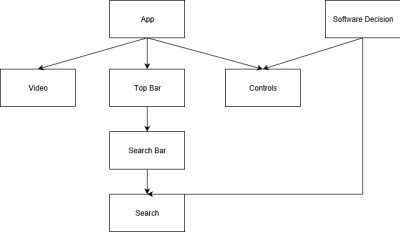
\includegraphics[width=0.7\textwidth]{UsesHierarchy.png}
\caption{Use hierarchy among modules}
\label{FigUH}
\end{figure}

%\section*{References}

\bibliographystyle {plainnat}
\bibliography {MG}

\end{document}